\documentclass[10pt]{article}
\usepackage[a4paper,margin=1.2cm]{geometry}
\usepackage{amsmath,amssymb}
\usepackage[dvipsnames]{xcolor}
\usepackage{multicol}
\usepackage{tikz}
\usetikzlibrary{arrows.meta,backgrounds,fit}
\pagestyle{empty}
\setlength{\parindent}{0pt}
\setlength{\parskip}{2pt}
\setlength{\abovedisplayskip}{3pt}
\setlength{\belowdisplayskip}{3pt}
\setlength{\abovedisplayshortskip}{2pt}
\setlength{\belowdisplayshortskip}{2pt}

\newcommand{\pd}[2]{\frac{\partial #1}{\partial #2}}
\newcommand{\into}{_{\leftarrow}}
\newcommand{\out}{^{\rightarrow}}
\newcommand{\Ey}[1]{\textcolor{BrickRed}{\pd{E_k}{y_{#1}}}}
\newcommand{\hsec}[1]{\par\vspace{4pt}{\large\bfseries #1}\par\vspace{1pt}\hrule\vspace{3pt}}

\begin{document}
\begin{center}
  {\LARGE\bfseries Backpropagation -- derivation}
\end{center}

\hsec{1\quad Notation}
\begin{multicols}{2}
\begin{tabular}{@{}ll@{}}
$X,Y\subseteq Z$ & input, output, all neurons \\
$\ell=0,\dots,L$ & layers;\; $X$ = layer $0$,\; $Y$ = layer $L$ \\
$\xi_j$ & inner potential of $j$ \\
$y_j$ & output of $j$;\; $y_0=1$,\; $0\notin Z$ \\
$w_{ji}$ & weight $i\to j$;\; $w_{j0}=b_j$ (bias) \\
$\sigma_j$ & activation of $j$ (differentiable)
\end{tabular}

\begin{tabular}{@{}ll@{}}
$j\into$ & $\{i : i\to j\}$ = layer $\ell-1$ $\cup\,\{0\}$ ($j$ in layer $\ell$) \\
$j\out$ & $\{r : j\to r\}$ = layer $\ell+1$ \\
$\mathcal T$ & $\{(\vec x_k,\vec d_k)\mid k=1,\dots,n\}$ \\
$d_{kj}$ & desired output of $j\in Y$ for $\vec x_k$ \\
$\mathcal B,\ p$ & minibatch of samples,\; $p=|\mathcal B|$ \\
$\varepsilon(t)$ & learning rate in step $t$,\; $0<\varepsilon(t)\le 1$
\end{tabular}
\end{multicols}

\hsec{2\quad Forward pass, error, update}
\[
\xi_j=\sum_{i\in j\into} w_{ji}\,y_i,\qquad
y_j=\sigma_j(\xi_j)=y_j(\vec w,\vec x_k)\quad(\text{layer by layer } \ell=1,\dots,L)
\]
\[
E_k(\vec w)=\tfrac12\sum_{j\in Y}\bigl(y_j(\vec w,\vec x_k)-d_{kj}\bigr)^2,\qquad
E(\vec w)=\frac1p\sum_{k\in\mathcal B} E_k(\vec w),\qquad
\textcolor{ForestGreen}{\pd{E}{w_{ji}}}=\frac1p\sum_{k\in\mathcal B}\textcolor{blue}{\pd{E_k}{w_{ji}}}
\]
\[
\text{step: } w_{ji}^{(t+1)}=w_{ji}^{(t)}-\varepsilon(t)\,\pd{E}{w_{ji}}(\vec w^{(t)})
\;\Leftrightarrow\;\vec w^{(t+1)}=\vec w^{(t)}-\varepsilon(t)\nabla E(\vec w^{(t)})
\]

\hsec{3\quad Derivation, layer by layer}
\textbf{(a) Any weight $w_{ji}$:}
\[
\textcolor{blue}{\pd{E_k}{w_{ji}}}
=\Ey{j}\cdot\pd{y_j}{w_{ji}}
=\Ey{j}\cdot\textcolor{ForestGreen}{\pd{y_j}{\xi_j}}\cdot\textcolor{Brown}{\pd{\xi_j}{w_{ji}}}
=\boxed{\Ey{j}\cdot\sigma_j'(\xi_j)\cdot y_i}
\qquad\text{bias } (i=0,\ y_0=1)\text{: }\
\pd{E_k}{w_{j0}}=\Ey{j}\cdot\sigma_j'(\xi_j)
\]
\[
\textcolor{ForestGreen}{\pd{y_j}{\xi_j}}=\pd{\sigma_j(\xi_j)}{\xi_j}=\sigma_j'(\xi_j),
\qquad
\textcolor{Brown}{\pd{\xi_j}{w_{ji}}}=\pd{\bigl(\sum_{r\in j\into}w_{jr}y_r\bigr)}{w_{ji}}=y_i
\]
\textbf{(b) Output layer $L$, $j\in Y$:}
\[
\Ey{j}=\pd{\bigl(\frac12\sum_{r\in Y}(y_r-d_{kr})^2\bigr)}{y_j}=\boxed{y_j-d_{kj}}
\]
\textbf{(c) Hidden layer $\ell$, $j\in Z\setminus(X\cup Y)$} ($r\in j\out$ already computed):
\[
\Ey{j}=\sum_{r\in j\out}\Ey{r}\cdot\pd{y_r}{y_j}
=\sum_{r\in j\out}\Ey{r}\cdot\textcolor{ForestGreen}{\pd{y_r}{\xi_r}}\cdot\textcolor{Brown}{\pd{\xi_r}{y_j}}
=\boxed{\sum_{r\in j\out}\Ey{r}\cdot\sigma_r'(\xi_r)\cdot w_{rj}}
\]
\[
\textcolor{ForestGreen}{\pd{y_r}{\xi_r}}=\pd{\sigma_r(\xi_r)}{\xi_r}=\sigma_r'(\xi_r),
\qquad
\textcolor{Brown}{\pd{\xi_r}{y_j}}=\pd{\bigl(\sum_{s\in r\into}w_{rs}y_s\bigr)}{y_j}=w_{rj}
\]

\hsec{4\quad Activations}
\textbf{(d) Logistic}:\;
$\sigma(\xi)=\dfrac{1}{1+e^{-\xi}}$,\quad
$\sigma'(\xi)=\dfrac{e^{-\xi}}{(1+e^{-\xi})^2}=\sigma(\xi)\bigl(1-\sigma(\xi)\bigr)$
\;$\Rightarrow$\; $\boxed{\sigma_j'(\xi_j)=y_j(1-y_j)}$.

\textbf{(e) ReLU}:\;
$\sigma(\xi)=\max(0,\xi)$,\quad
$\boxed{\sigma_j'(\xi_j)=[\,\xi_j>0\,]}$ \;($0$ at $\xi_j=0$).

\hsec{5\quad Algorithm (one step)}
\begin{minipage}[t]{0.55\textwidth}
$\mathcal E_{ji}:=0$;\quad \textbf{for} $k\in\mathcal B$:
\begin{enumerate}\setlength{\itemsep}{1pt}\setlength{\topsep}{2pt}
  \item \textbf{forward:} $\xi_j,\ y_j=y_j(\vec w,\vec x_k)$ for all $j$
  \item \textbf{backward:} $\Ey{j}$ for all $j$, layers $L\to1$, by (b), (c)
  \item $\displaystyle \pd{E_k}{w_{ji}}:=\Ey{j}\cdot\sigma_j'(\xi_j)\cdot y_i$ by (a)
  \item $\mathcal E_{ji}:=\mathcal E_{ji}+\frac1p\pd{E_k}{w_{ji}}$
\end{enumerate}
Then $\mathcal E_{ji}=\pd{E}{w_{ji}}$; update $w_{ji}$. Cost: $O(|\vec w|\cdot p)$.
\end{minipage}\hfill
\begin{minipage}[t]{0.43\textwidth}
\vspace{-6pt}
\centering
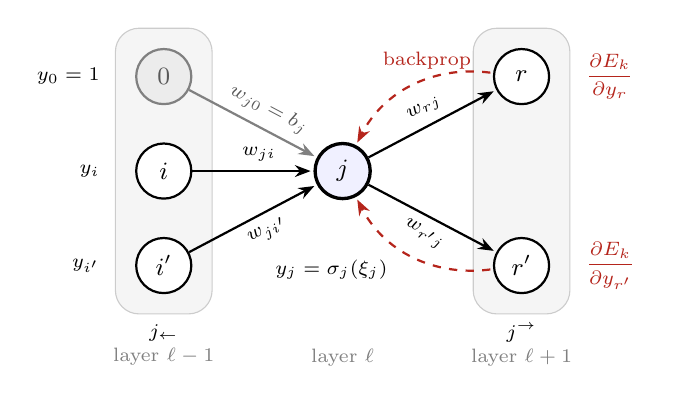
\begin{tikzpicture}[
  x=1.42cm,y=1cm,
  n/.style={circle,draw,thick,minimum size=7mm,inner sep=0pt,font=\small,fill=white},
  bias/.style={n,draw=gray,fill=gray!15,text=gray!70!black},
  fwd/.style={-{Stealth[length=2mm]},thick,shorten >=1pt},
  bwd/.style={-{Stealth[length=2mm]},BrickRed,dashed,thick,shorten >=1pt,shorten <=1pt},
  ann/.style={font=\scriptsize},
  set/.style={rounded corners=3mm,fill=gray!8,draw=gray!40},
  layer/.style={font=\scriptsize,gray}]
  % neurons
  \node[bias] (0)  at (0, 1.5) {$0$};
  \node[n]    (i)  at (0, 0.3) {$i$};
  \node[n]    (i2) at (0,-0.9) {$i'$};
  \node[n,very thick,fill=blue!6] (j) at (1.6,0.3) {$j$};
  \node[n]    (r)  at (3.2, 1.5) {$r$};
  \node[n]    (r2) at (3.2,-0.9) {$r'$};
  % sets (behind)
  \begin{scope}[on background layer]
    \node[set,fit=(0)(i2),name=lset,inner sep=2.5mm,label={[ann,align=center]below:$j\into$\\[1pt]{\color{gray}layer $\ell-1$}}] {};
    \node[set,fit=(r)(r2),name=rset,inner sep=2.5mm,label={[ann,align=center]below:$j\out$\\[1pt]{\color{gray}layer $\ell+1$}}] {};
  \end{scope}
  % forward
  \draw[fwd,gray] (0) -- node[ann,pos=0.55,sloped,above,text=gray!70!black]{$w_{j0}=b_j$} (j);
  \draw[fwd] (i)  -- node[ann,pos=0.55,above]{$w_{ji}$} (j);
  \draw[fwd] (i2) -- node[ann,pos=0.55,sloped,below]{$w_{ji'}$} (j);
  \draw[fwd] (j) -- node[ann,pos=0.5,sloped,above]{$w_{rj}$} (r);
  \draw[fwd] (j) -- node[ann,pos=0.5,sloped,below]{$w_{r'j}$} (r2);
  % backward
  \draw[bwd] (r)  to[bend right=35] node[ann,above,text=BrickRed,pos=0.4]{backprop} (j);
  \draw[bwd] (r2) to[bend left=35] (j);
  % annotations
  \node[ann,left=2pt]  at (lset.west |- 0) {$y_0=1$};
  \node[ann,left=2pt]  at (lset.west |- i) {$y_i$};
  \node[ann,left=2pt]  at (lset.west |- i2) {$y_{i'}$};
  \node[ann] at (1.5,-0.95) {$y_j=\sigma_j(\xi_j)$};
  \node[ann,text=BrickRed,right=2pt] at (rset.east |- r)  {$\dfrac{\partial E_k}{\partial y_r}$};
  \node[ann,text=BrickRed,right=2pt] at (rset.east |- r2) {$\dfrac{\partial E_k}{\partial y_{r'}}$};
  % layer of j, level with the set labels
  \path (i2.south) ++(0,-0.25) coordinate (lb);
  \node[ann,align=center,anchor=north] at (j |- lb) {\phantom{$j\out$}\\[1pt]{\color{gray}layer $\ell$}};
\end{tikzpicture}
\end{minipage}

\end{document}
